The objective is to investigate if voids can be detected using a single projection. The quality control procedure can be sped up if defect detection can be done in projection space rather than reconstruction space. An experiment was conducted where a test sample was additively manufactured with purposely designed voids. This was done by comparing a projection of the test sample with the simulation of that projection as if the voids were not there. The simulated projections were produced by using software called \emph{aRTist} \citep{bellon2007artist, jaenisch2008artist, bellon2012radiographic}. Any disagreement in the comparison can suggest evidence of a defect.

This chapter describes the apparatus used to manufacture the test sample and obtaining the projections. There is also a discussion, at the end of the chapter, on shading correction which was used to remove panel and x-ray spot effects from the projections.

Many figures presented here were given by engineers concerning the experiment or by the manufacturer. Figures with no error bars were rounded to an appropriate number of significant figures.

\section{Apparatus}

The test object is a cuboid (\SI{40.0}{\milli\metre} $\times$ \SI{40.0}{\milli\metre} $\times$ \SI{60.0}{\milli\metre}) with voids. The voids were of diameters \SI{2.4}{\milli\metre}, \SI{1.2}{\milli\metre}, \SI{0.6}{\milli\metre} and \SI{0.3}{\milli\metre}. 6 voids for each diameter were designed in the CAD model. Voids with diameters \SI{2.4}{\milli\metre} and \SI{0.6}{\milli\metre} were regularly arranged, the other ones were arranged irregularly. The CAD model of the test sample is shown in Figure \ref{fig:inference_testObject}.

\begin{figure}
  \centering
  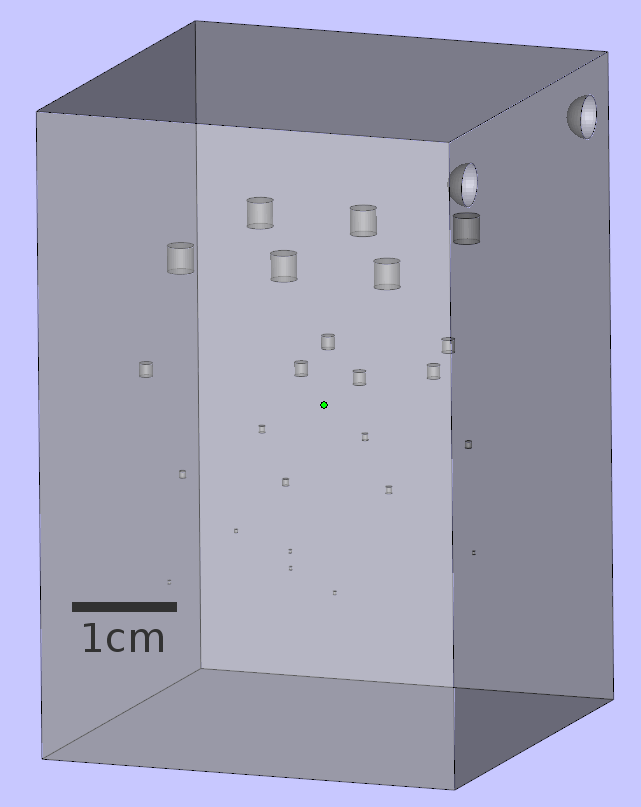
\includegraphics[width=0.4\textwidth]{../figures/inference/TestObject.png}
  \caption{The CAD model of the test sample. The scale is approximate.}
  \label{fig:inference_testObject}
\end{figure}

The \emph{Fortus 400mc (Stratasys, US)} was used to manufacture the test object made of plastic (acrylonitrile butadiene styrene or ABS). The precision of the manufacturing was in the order of $\pm\SI{0.1}{\milli\metre}$ \citep{hanseen2013fortus}.

X-ray projections were obtained using the \emph{Nikon XT H LC 225/320} x-ray CT scanner (\emph{Nikon Metrology, UK}) together with a \emph{Perkin Elmer XRD 1621 (Perkin Elmer, US)} detector. The target material in the x-ray tube was tungsten. The detector was made up of 2 rows and 16 columns of panels and together has dimensions of $\SI{409.6}{\milli\metre}\times\SI{409.6}{\milli\metre}$ which produced a 16-bit projection of $\SI{2048}{\pixel}\times\SI{2048}{\pixel}$ in size \citep{perkinelmer2006xrd}. Therefore, the scale of each pixel is $\SI{200.0}{\micro\metre\per\pixel}$. The projections were cropped to $\SI{2000}{\pixel}\times\SI{2000}{\pixel}$ to remove boundary effects. The gain and offset were adjusted by the engineers to produce a projection with good contrast and negligible penumbra effect. Each pixel has a grey value in units of analogue to digital units (\SI{}{\adu}).

Greyscale projections were taken in addition to the projection of the test object. These are projections with nothing between the source and the detector, obtained with the x-ray tube at different powers. The power was varied by fixing the potential difference and varying the current. The greyscale projections were used for calibration such as shading correction. The greyscale projection with the x-ray turned off is called the black image. The greyscale projection with the x-ray set up the same when obtaining the test sample projection is called the white image.

Replicate test sample projections and greyscale projections were obtained by repeating the acquisition. These replicated projections were used to study the noise observed in the projections.

A \SI{0.35}{\milli\metre} copper filter was used to tackle beam hardening.

\emph{aRTist} was used to simulate the test object projection and all greyscale projections except for the black image. The black image was simulated by producing a uniform image with a grey value the mean over the obtained black image. The engineers used numerical methods to align the simulated projection with the obtained projection.

\section{Datasets}

Two datasets were collected and named \texttt{AbsNoFilter} and \texttt{AbsFilter}. They contain replicate projections of the test sample at two different angles, named $\ang{30}$ and $\ang{120}$, as well as replicate greyscale projections. To investigate the effects of beam hardening, no x-ray filter was used in \texttt{AbsNoFilter} and a filter was used in \texttt{AbsFilter}.

The properties of each dataset are shown in Table \ref{table:data_dataset}. These include the properties of the x-ray tube, the XCT apparatus and what powers were used in the greyscale projections. A sample of the obtained, simulated and greyscale projections from the datasets \texttt{AbsNoFilter} and \texttt{AbsFilter} are shown in Figures \ref{fig:data_AbsNoFilter} and \ref{fig:data_AbsFilter} respectively.

\begin{sidewaystable}
\centering
\begin{tabular}{l|cc}
                                                       & \multicolumn{2}{c}{Dataset name}                      \\
                                                       & \texttt{AbsNoFilter} & \texttt{AbsFilter}             \\ \hline
potential difference (\SI{}{\kilo\volt})               & 80                   & 80                             \\
power (\SI{}{\watt})                                   & 36                   & 20                             \\
filter                                                 & no filter            & \SI{0.35}{\milli\metre} copper \\
time exposure (\SI{}{\milli\second})                   & 708                  & 500                            \\
distance from source to object (\SI{}{\milli\metre})   & 217                  & 168                            \\
distance from source to detector (\SI{}{\milli\metre}) & 1178                 & 876                            \\
number of replications for each angle                  & 100                  & 20                             \\ \hline
powers used for greyscale projections (\SI{}{\watt})   & 0.0                  & 0.0                            \\
\multicolumn{1}{c|}{\vdots}                            & 10                   & 5.0                            \\
\multicolumn{1}{c|}{\vdots}                            & 18                   & 10                             \\
\multicolumn{1}{c|}{\vdots}                            & 28                   & 15                             \\
\multicolumn{1}{c|}{\vdots}                            & 36                   & 20                             \\
number of replications for each power                  & 20                   & 20                             
\end{tabular}
\caption{Properties of the two datasets obtained for the experiment.}
\label{table:data_dataset}
\end{sidewaystable}

\begin{figure}[p]
  \centering
  \centerline{
    \begin{subfigure}[b]{\subSize}
      \includegraphics[width=\textwidth]{../figures/data/AbsNoFilterDeg30.eps}
      \caption{Obtained projection at \SI{36}{\watt}}
    \end{subfigure}
    \begin{subfigure}[b]{\subSize}
      \includegraphics[width=\textwidth]{../figures/data/AbsNoFilterDeg30_sim.eps}
      \caption{Simulated projection at \SI{36}{\watt}}
    \end{subfigure}
  }
  \centerline{
    \begin{subfigure}[b]{\subSize}
      \includegraphics[width=\textwidth]{../figures/data/AbsNoFilter_calibration1.eps}
      \caption{Greyscale projection at \SI{0}{\watt}}
    \end{subfigure}
    \begin{subfigure}[b]{\subSize}
      \includegraphics[width=\textwidth]{../figures/data/AbsNoFilter_calibration5.eps}
      \caption{Greyscale projection at \SI{36}{\watt}}
    \end{subfigure}
  }
  \caption{\texttt{AbsNoFilter} projections at \ang{30}. The colour scales are in units of \SI{}{\adu}.}
  \label{fig:data_AbsNoFilter}
\end{figure}

\begin{figure}[p]
  \centering
  \centerline{
    \begin{subfigure}[b]{\subSize}
      \includegraphics[width=\textwidth]{../figures/data/AbsFilterDeg30.eps}
      \caption{Obtained projection at \SI{20}{\watt}}
    \end{subfigure}
    \begin{subfigure}[b]{\subSize}
      \includegraphics[width=\textwidth]{../figures/data/AbsFilterDeg30_sim.eps}
      \caption{Simulated projection at \SI{20}{\watt}}
    \end{subfigure}
  }
  \centerline{
    \begin{subfigure}[b]{\subSize}
      \includegraphics[width=\textwidth]{../figures/data/AbsFilter_calibration1.eps}
      \caption{Greyscale projection at \SI{0}{\watt}}
    \end{subfigure}
    \begin{subfigure}[b]{\subSize}
      \includegraphics[width=\textwidth]{../figures/data/AbsFilter_calibration5.eps}
      \caption{Greyscale projection at \SI{20}{\watt}}
    \end{subfigure}
  }
  \caption{\texttt{AbsFilter} projections at \ang{30}. The colour scales are in units of \SI{}{\adu}.}
  \label{fig:data_AbsFilter}
\end{figure}

The projections show the test sample, but, with panel and spot effects. The structure of the 32 panels are predominate in the black image, in particular, this was observed by \cite{yang2009evaluation} as well. This is concerning because systematic errors could be introduced as a result of the panel effects in the black image. A black image should be flat because the detector is exposed only to background radiation. The x-ray spot can be observed, in particular, in the white image, and this is the result of using a cone beam.

\afterpage{\clearpage}

\section{Shading Correction}

Shading correction, also known as flat field correction, aims to eliminate any spatial variation in sensitivity, observed in the projections, as a result from panel effects, spot effects and other artefacts. Shading correction is done by using the greyscale projections and examining how the grey values respond to different powers for different pixels. For example, the black and white image can be used to correct the projections using
\begin{equation}
U_{x,y} = \dfrac{N_{x,y}-\text{black}_{x,y}}{\text{white}_{x,y}-\text{black}_{x,y}}\times B+A
\label{eq:data_shadingCorrectionOld}
\end{equation}
where $N_{x,y}$ is the obtained projection, $U_{x,y}$ is the shading corrected projection and $A$ and $B$ are some user defined constants \citep{young2000shading, munzenmayer2003enhancing}. This can be extended to include more greyscale projections by modelling the grey value to respond linearly to the power of the x-ray source \citep{seibert1998flat}. More generally, shading correction can be expressed as
\begin{equation}
U_{x,y} = \beta_{x,y} N_{x,y} + \alpha_{x,y}
\end{equation}
where $\alpha_{x,y}$ and $\beta_{x,y}$ are some spatially varying functions \citep{munzenmayer2003enhancing}. This model has limitations because $\alpha_{x,y}$ and $\beta_{x,y}$ may depend on the energy of each photon, thus beam hardening could cause inaccuracies in shading correction \citep{davidson2003limitations}. Other methods include minimising the entropy of the projection while constraining $\alpha_{x,y}$ and $\beta_{x,y}$ to be some parametric function \citep{likar2000retrospective} and using a low pass filter to remove low spatial frequencies from the projections \citep{young2000shading, munzenmayer2003enhancing}.

In this section, the shading correction in \cite{seibert1998flat} is presented in a form without any user-defined constants. The shading correction was experimented to investigate its performance when shading correcting greyscale projections.

\subsection{Proposed Shading Correction}

Let $S_{x,y}(P)$ be the greyscale projection when exposed to x-rays produced by an x-ray tube with power $P$ for some fixed time exposure $\tau$. $S_{x,y}(P)$ may be averaged over replications. Let $x=1,2,3,\dotsc, W$ and $y=1,2,3,\dotsc,H$. Let $N_{x,y}$ be the obtained projection of the test sample when exposed to x-rays produced by an x-ray tube with power $P_\text{proj}$ for some fixed time exposure $\tau$. The black and white image can be expressed as $\text{black}_{x,y}=S_{x,y}(0)$ and $\text{white}_{x,y}=S_{x,y}(P_\text{proj})$ respectively. The power was varied by fixing the potential difference and varying the current of the x-ray tube.

The shading free image is not known, but it is expected that the shading corrected greyscale projection should be flat with some noise. In other words, all pixels in a shading corrected greyscale projection should have grey values with the same expectation $\mu_{S}(P)$ and same variance $\sigma_{S}^2(P)$. Suppose $\mu_{S}(P)$ was estimated using the within projection mean
\begin{equation}
\overline{S}(P) = \dfrac{1}{\text{WH}}
\sum_{x=1}^W\sum_{y=1}^H S_{x,y}(P) \ .
\end{equation}
Consider a pixel at $(x,y)$, shading correction was done by fitting a linear regression on
\begin{equation}
\overline{S}(P) = \beta_{x,y} S_{x,y}(P) + \alpha_{x,y} \quad(+\varepsilon)
\end{equation}
for $P\in \mathbb{P}$ where $\mathbb{P} = \left\{0,P_1,P_2,\cdots, P_\text{proj}\right\}$ are the powers used for the greyscale projections. $\varepsilon$ is a random variable and an error term, it is included for formality purposes. Let $b_{x,y}$ and $a_{x,y}$ be the estimated parameters of $\beta_{x,y}$ and $\alpha_{x,y}$ from the linear regression respectively. Given a projection $N_{x,y}$, the shading corrected projection $U_{x,y}$ is
\begin{equation}
U_{x,y} = b_{x,y} N_{x,y} + a_{x,y} \ .
\end{equation}
In full, the equations for $b_{x,y}$ and $a_{x,y}$ are given as
\begin{equation}
b_{x,y} = \dfrac{
  \sum_{P\in\mathbb{P}}(S_{x,y}(P) - \overline{S}_{x,y})(\overline{S}(P) - \overline{S})
}{
  \sum_{P\in\mathbb{P}}(S_{x,y}(P) - \overline{S}_{x,y})^2
}
\end{equation}
and
\begin{equation}
a_{x,y} = \overline{S} - b_{x,y}\overline{S}_{x,y}
\end{equation}
where $\overline{S}_{x,y}$ is the between projection mean
\begin{equation}
\overline{S}_{x,y} = \dfrac{1}{|\mathbb{P}|}\sum_{P\in\mathbb{P}}S_{x,y}(P)
\end{equation}
and $\overline{S}$ is the global mean
\begin{equation}
\overline{S} = \dfrac{1}{|\mathbb{P}|}\sum_{P\in\mathbb{P}}\overline{S}(P) \ .
\end{equation}
This type of shading correction shall be referred to as linear shading correction. Expressing shading correction in this way has the advantage that there are no user defined constants.

An example of the linear regression is shown in Figure \ref{fig:data_shadingCorrectionExample_gainMap} where 3 random pixels were chosen for illustration. By plotting the within projection mean versus the grey value for a particular pixel, a linear relationship can be observed. The gradient varied for different pixels which correspond to different sensitivities. The resulting shading correction for the \texttt{AbsNoFilter} projection is shown in Figure \ref{fig:data_shadingCorrectionExample_image}. It can be observed that the shading correction removed the panel and spot effects from the background and test sample.

\begin{figure}
  \centering
  \centerline{
    \begin{subfigure}[b]{\subSize}
      \includegraphics[width=\textwidth]{../figures/data/shadingCorrectionExample_interpolation.eps}
      \caption{Linear regression}
    \end{subfigure}
    \begin{subfigure}[b]{\subSize}
      \includegraphics[width=\textwidth]{../figures/data/shadingCorrectionExample_gradient_linear.eps}
      \caption{$b_{x,y}$}
    \end{subfigure}
  }
  \caption{For each pixel, a linear regression was fitted on the within projection mean versus the pixel's grey value. The \texttt{AbsNoFilter} dataset was used. 3 random pixels were used to illustrate this in a). b) shows the fitted gradient for all pixels.}
  \label{fig:data_shadingCorrectionExample_gainMap}
\end{figure}

\begin{figure}
  \centering
  \centerline{
    \begin{subfigure}[b]{\subSize}
      \includegraphics[width=\textwidth]{../figures/data/shadingCorrectionExample_image_null.eps}
      \caption{No shading correction}
    \end{subfigure}
    \begin{subfigure}[b]{\subSize}
      \includegraphics[width=\textwidth]{../figures/data/shadingCorrectionExample_image_linear.eps}
      \caption{Linear shading correction}
    \end{subfigure}
  }
  \caption{Projection of \texttt{AbsNoFilter} at \ang{30} with and without shading correction. The colour scales are in units of \SI{}{\adu}.}
  \label{fig:data_shadingCorrectionExample_image}
\end{figure}

A variation of the shading correction which uses only the black and white image such that $\mathbb{P}=\left\{0, P_\text{proj}\right\}$ shall be known as black/white (BW) shading correction.

\subsection{Exploratory Analysis}

It was investigated if shading correction on a greyscale projection results in an image which is flat with some noise. To avoid overfitting, one greyscale projection from each power was held out and used to fit the parameters of the shading correction. Shading correction was then used on the unused greyscale projections in this exploratory analysis.

Figure \ref{fig:data_shadingCorrectionExample_greyvaluePower} shows the grey values in each greyscale projections before and after shading correction. The sensitivity of the pixels, which corresponds to the gradient in units of \SI{}{\adu\per\watt}, became more consistent with shading correction. This should imply that pixels should respond similarly to each other for varying power with shading correction

\begin{figure}
  \centerline{
    \begin{subfigure}[b]{\subSize}
      \includegraphics[width=\textwidth]{../figures/data/shadingCorrectionExample_power_null.eps}
      \caption{No shading correction}
    \end{subfigure}
    \begin{subfigure}[b]{\subSize}
      \includegraphics[width=\textwidth]{../figures/data/shadingCorrectionExample_power_linear.eps}
      \caption{Linear shading correction}
    \end{subfigure}
  }
  \caption{Grey values in the greyscale projections before and after shading correction using the \texttt{AbsNoFilter} dataset. The boxplots summarise all $2\,000\times2\,000$ pixels in a projection.}
  \label{fig:data_shadingCorrectionExample_greyvaluePower}
\end{figure}

The \texttt{AbsNoFilter} black and white images before and after shading correction are shown in Figure \ref{fig:data_shadingCorrectionExample_greyscale}. The flatness of the image can be shown using a profile plot, this is a plot of the grey values along a column or row, an example shown in Figure \ref{fig:data_oddEven}. The figure shows that the shading uncorrected black image was not flat but a remarkable structure was observed by plotting the odd rows and even rows separately. Such a plot shows that the grey values depend on neighbouring pixels, where the majority of pixels on even rows have grey values larger than pixels above and below it. Perhaps this is caused by the read-out structure in the detector.

The BW shading corrected black and white image appeared uniform but there is some structure in the linear shading correction. By giving linear shading correction various greyscale projections, it attempts to generalise to a range of powers, thus may struggle at shading correcting the black and white images.

\begin{figure}
  \centerline{
    \begin{subfigure}[b]{\subSize}
      \includegraphics[width=\textwidth]{../figures/data/shadingCorrectionExample_black_null.eps}
      \caption{Black - No shading correction}
    \end{subfigure}
    \begin{subfigure}[b]{\subSize}
      \includegraphics[width=\textwidth]{../figures/data/shadingCorrectionExample_white_null.eps}
      \caption{White - No shading correction}
    \end{subfigure}
  }
  \centerline{
    \begin{subfigure}[b]{\subSize}
      \includegraphics[width=\textwidth]{../figures/data/shadingCorrectionExample_black_bw.eps}
      \caption{Black - BW shading correction}
    \end{subfigure}
    \begin{subfigure}[b]{\subSize}
      \includegraphics[width=\textwidth]{../figures/data/shadingCorrectionExample_white_bw.eps}
      \caption{White - BW shading correction}
    \end{subfigure}
  }
  \centerline{
    \begin{subfigure}[b]{\subSize}
      \includegraphics[width=\textwidth]{../figures/data/shadingCorrectionExample_black_linear.eps}
      \caption{Black - Linear shading correction}
    \end{subfigure}
    \begin{subfigure}[b]{\subSize}
      \includegraphics[width=\textwidth]{../figures/data/shadingCorrectionExample_white_linear.eps}
      \caption{White - Linear shading correction}
    \end{subfigure}
  }
  \caption{The black and white images before and after shading correction from the \texttt{AbsNoFilter} dataset. The colour scales are in units of \SI{}{\adu}.}
  \label{fig:data_shadingCorrectionExample_greyscale}
\end{figure}

\begin{figure}
  \centerline{
    \begin{subfigure}[b]{\textwidth}
      \includegraphics[width=\subSize]{../figures/data/oddEvenPlot1_null.eps}
      \includegraphics[width=\subSize]{../figures/data/oddEvenPlot2_null.eps}
      \caption{No shading correction}
    \end{subfigure}
  }
  \centerline{
    \begin{subfigure}[b]{\textwidth}
      \includegraphics[width=\subSize]{../figures/data/oddEvenPlot1_bw.eps}
      \includegraphics[width=\subSize]{../figures/data/oddEvenPlot2_bw.eps}
      \caption{BW shading correction}
    \end{subfigure}
  }
  \centerline{
    \begin{subfigure}[b]{\textwidth}
      \includegraphics[width=\subSize]{../figures/data/oddEvenPlot1_linear.eps}
      \includegraphics[width=\subSize]{../figures/data/oddEvenPlot2_linear.eps}
      \caption{linear shading correction}
    \end{subfigure}
  }
  \caption{Left shows the profile plot of an \texttt{AbsNoFilter} black image at $(879,y)$ using various shading corrections. Right shows two curves for odd and even $y$.}
  \label{fig:data_oddEven}
\end{figure}

\subsection{ANOVA}

An experiment was conducted to quantify the performance of the different types of shading correction. Applying shading correction on the greyscale image should remove effects from the panels and the spot, leaving a flat noisy image with no spatial structure. The variance within a pixel and across replications should be similar to the variance between pixels within a replication if shading correction flattens the greyscale images.

In each dataset, there are 20 replicated greyscale images for each power. One randomly selected replication from each power was assigned to the training set and used to calibrate the shading correction. The remaining images were assigned to the test set and the shading correction was applied to each image.

For each power, the within and between pixel variance was calculated. Let $U_{x,y}^{(j)}(P)$ be the shading corrected greyscale image in the test set with power $P$ for $j=1,2,\dotsc,m$ replicates. The within and between pixel variance are
\begin{equation}
s_\mathrm{w}^2(P)=\dfrac{1}{WH(m-1)}
  \sum_{x=1}^{W}\sum_{y=1}^{H}\sum_{j=1}^{m}
  \left(
    U_{x,y}^{(j)}(P) - \overline{U}_{x,y}(P)
  \right)^2
\end{equation}
and
\begin{equation}
s_\mathrm{b}^2(P)=\dfrac{m}{WH-1}
  \sum_{x=1}^{W}\sum_{y=1}^{H}
  \left(
    \overline{U}_{x,y}(P) - \overline{U}(P)
  \right)^2
\end{equation}
respectively where
\begin{equation}
  \overline{U}_{x,y}(P) = \dfrac{1}{m}\sum_{j=1}^{m}U_{x,y}^{(j)}(P)
\end{equation}
and
\begin{equation}
  \overline{U}(P) = \dfrac{1}{WH}\sum_{x=1}^{W}\sum_{y=1}^{H}\overline{U}_{x,y}(P)
  \ .
\end{equation}
In this specific experiment, $W=2000$, $H=2000$ and $m=19$. The $F$ statistic is
\begin{equation}
F(P)=\dfrac{s_\mathrm{b}^2(P)}{s_\mathrm{w}^2(P)}
\end{equation}
and it should be about one if the within and between pixel variances are similar. The experiment was repeated 100 times by reallocating the training and test set.

\begin{figure}[p]
  \centering
  \centerline{
    \begin{subfigure}[b]{\subSize}
      \includegraphics[width=\textwidth]{../figures/data/ShadingCorrectionAnovaAbsNoFilter_null.eps}
      \caption{No shading correction}
    \end{subfigure}
    \begin{subfigure}[b]{\subSize}
      \includegraphics[width=\textwidth]{../figures/data/ShadingCorrectionAnovaAbsNoFilter_bw.eps}
      \caption{BW shading correction}
    \end{subfigure}
  }
  \centerline{
    \begin{subfigure}[b]{\subSize}
      \includegraphics[width=\textwidth]{../figures/data/ShadingCorrectionAnovaAbsNoFilter_linear.eps}
      \caption{Linear shading Correction}
    \end{subfigure}
    \begin{subfigure}[b]{\subSize}
      \includegraphics[width=\textwidth]{../figures/data/ShadingCorrectionAnovaAbsNoFilter_FStatistic.eps}
      \caption{$F$ statistic}
    \end{subfigure}
  }
  \caption{One randomly selected greyscale image from each power was used to train the shading correction which was then applied to the remaining of the greyscale projections. The within and between pixel variance were estimated and used to calculate a $F$ statistic for each power. The experiment was repeated by reselecting the greyscale projections used for training the shading correction.  The boxplots represent the 100 repeats. The \texttt{AbsNoFilter} dataset was used here.}
  \label{fig:data_anovaAbsNoFilter}
\end{figure}

\begin{figure}[p]
  \centering
  \centerline{
    \begin{subfigure}[b]{\subSize}
      \includegraphics[width=\textwidth]{../figures/data/ShadingCorrectionAnovaAbsFilter_null.eps}
      \caption{No shading correction}
    \end{subfigure}
    \begin{subfigure}[b]{\subSize}
      \includegraphics[width=\textwidth]{../figures/data/ShadingCorrectionAnovaAbsFilter_bw.eps}
      \caption{BW shading correction}
    \end{subfigure}
  }
  \centerline{
    \begin{subfigure}[b]{\subSize}
      \includegraphics[width=\textwidth]{../figures/data/ShadingCorrectionAnovaAbsFilter_linear.eps}
      \caption{Linear shading Correction}
    \end{subfigure}
    \begin{subfigure}[b]{\subSize}
      \includegraphics[width=\textwidth]{../figures/data/ShadingCorrectionAnovaAbsFilter_FStatistic.eps}
      \caption{$F$ statistic}
    \end{subfigure}
  }
  \caption{One randomly selected greyscale image from each power was used to train the shading correction which was then applied to the remaining of the greyscale projections. The within and between pixel variance were estimated and used to calculate a $F$ statistic for each power. The experiment was repeated by reselecting the greyscale projections used for training the shading correction.  The boxplots represent the 100 repeats. The \texttt{AbsFilter} dataset was used here.}
  \label{fig:data_anovaAbsFilter}
\end{figure}

The results are shown in Figures \ref{fig:data_anovaAbsNoFilter} and \ref{fig:data_anovaAbsFilter} for the datasets \texttt{AbsNoFilter} and \texttt{AbsFilter} respectively. With shading correction, the within and between pixel variance became similar. A difference between BW and linear shading correction was that for the black image, the $F$ statistic is closer to one for BW shading correction compared with linear shading correction. For the rest of the powers, linear shading correction outperformed BW shading correction. This shows that linear shading correction generalises to powers between zero and $P_\text{proj}$. Since beam extinction is avoided, black grey values in the obtained projection should not be possible. As a result, the linear shading correction is recommended for its good performance for various powers.

Using the $F$ test from ANOVA was found to be too strict in this experiment. Under the hypothesis that the grey values all have the same mean and assume they are Normally distributed and i.i.d., then $F(P)\sim F_{WH-1, WH(m-1)}$. In this experiment, the 5\% critical value is 1.001 to 3 decimal places, this is too small for this analysis. This may be due to the grey values of the greyscale projections not satisfying the assumptions for the $F$ test, for example, they may not be i.i.d.

\subsection{Conclusion}

Shading correction is important because it removes any panel and spot effects from projections which may cause systematic errors in any statistical analysis. Shading correcting the greyscale projections visually produced a flat image but there was some spatial variation which was picked up by the between pixel variances in ANOVA.

Linear shading correction outperformed BW shading correction, in terms of ANOVA, on all greyscale projections except for the black image. This is because linear shading correction trains on greyscale projections of various powers and generalises to these powers. Linear shading correction is used throughout this thesis.

The variance of the greyscale projections was studied in this chapter. This is straightforward because the greyscale projections are flat images. The noise of a projection of a test sample is studied in the next chapter and this was done by modelling the grey value of each pixel as a compound Poisson random variable.